%%%%%%%%%%%%%%%%%%%%%%% file template.tex %%%%%%%%%%%%%%%%%%%%%%%%%
%
% This is a general template file for the LaTeX package SVJour3
% for Springer journals.          Springer Heidelberg 2010/09/16
%
% Copy it to a new file with a new name and use it as the basis
% for your article. Delete % signs as needed.
%
% This template includes a few options for different layouts and
% content for various journals. Please consult a previous issue of
% your journal as needed.
%
%%%%%%%%%%%%%%%%%%%%%%%%%%%%%%%%%%%%%%%%%%%%%%%%%%%%%%%%%%%%%%%%%%%
%
% First comes an example EPS file -- just ignore it and
% proceed on the \documentclass line
% your LaTeX will extract the file if required
%\begin{filecontents*}{example.eps}
%!PS-Adobe-3.0 EPSF-3.0
%%BoundingBox: 19 19 221 221
%%CreationDate: M
%\documentclass{svjour3}                     % onecolumn (standard format)
\documentclass{report}     % onecolumn (ditto)
%\documentclass[smallcondensed]{svjour3}       % onecolumn (second format)
%\documentclass[twocolumn]{svjour3}          % twocolumn
%
%\smartqed  % flush right qed marks, e.g. at end of proof
\usepackage[letterpaper, margin=0.9in]{geometry}
\usepackage{graphicx}
\usepackage{multirow}
\usepackage[authoryear,round]{natbib}
\usepackage{caption}
\usepackage{booktabs}
%\usepackage[sectionbib]{chapterbib}
\usepackage[usenames, dvipsnames]{color}   %May be necessary if you want to color links
\usepackage[hidelinks,linktoc=all]{hyperref}
\usepackage{textgreek}
\usepackage{mathpazo}
\usepackage{newtxtext,newtxmath,amsmath}
\usepackage[utf8]{inputenc}
\renewcommand{\arraystretch}{1.5}
\usepackage[
singlelinecheck=false 
]{caption}
\pagenumbering{gobble}


\makeatletter
\renewcommand*{\thetable}{\arabic{table}}
\renewcommand*{\thefigure}{\arabic{figure}}
\let\c@table\c@figure
\makeatother 

%\renewcommand{\figurename}{Online Resource}
%\usepackage[figurename=Online Resource]{caption}
\captionsetup[figure]{labelfont={bf},name={Online Resource},labelsep=space}
\captionsetup[table]{labelfont={bf},name={Online Resource},labelsep=space}
%\usepackage[labelfont=bf]{caption}
%
% \usepackage{mathptmx}      % use Times fonts if available on your TeX system
%
% insert here the call for the packages your document requires
%\usepackage{latexsym}
% etc.
%
% please place your own definitions here and don't use \def but
% \newcommand{}{}
%
% Insert the name of "your journal" with
% \journalname{myjournal}
%
\begin{document}

\title{Importance of sediment grain size to stocks and stability of organic carbon buried in seagrass soils \bigskip Supplementary material \bigskip}

% if too long for running head

\author{Jason L. Howard         \and
        Christian C. Lopes       \and
        Claudia I. Carri\'{o}n    \and
        Sara S. Wilson         \and
        James W. Fourqurean %etc.
}




% The correct dates will be entered by the editor


%\maketitle



\section*{Importance of sediment grain size to stocks and stability of organic carbon buried in seagrass soils}


\subsection*{Supplementary material \bigskip}
Jason L. Howard $\cdot$ Christian C. Lopes $\cdot$ Claudia I. Carri\'{o}n $\cdot$ Sara S. Wilson $\cdot$ James W. Fourqurean

%J.L. Howard $\cdot$ C.C. Lopes $\cdot$ C.I. Carri\'{o}n $\cdot$ Claudia I. Carri\'{o}n $\cdot$ Sara S. Wilson $\cdot$ James W. Fourqurean

\bigskip
\bigskip

\begin{figure}[h]
  \centering
   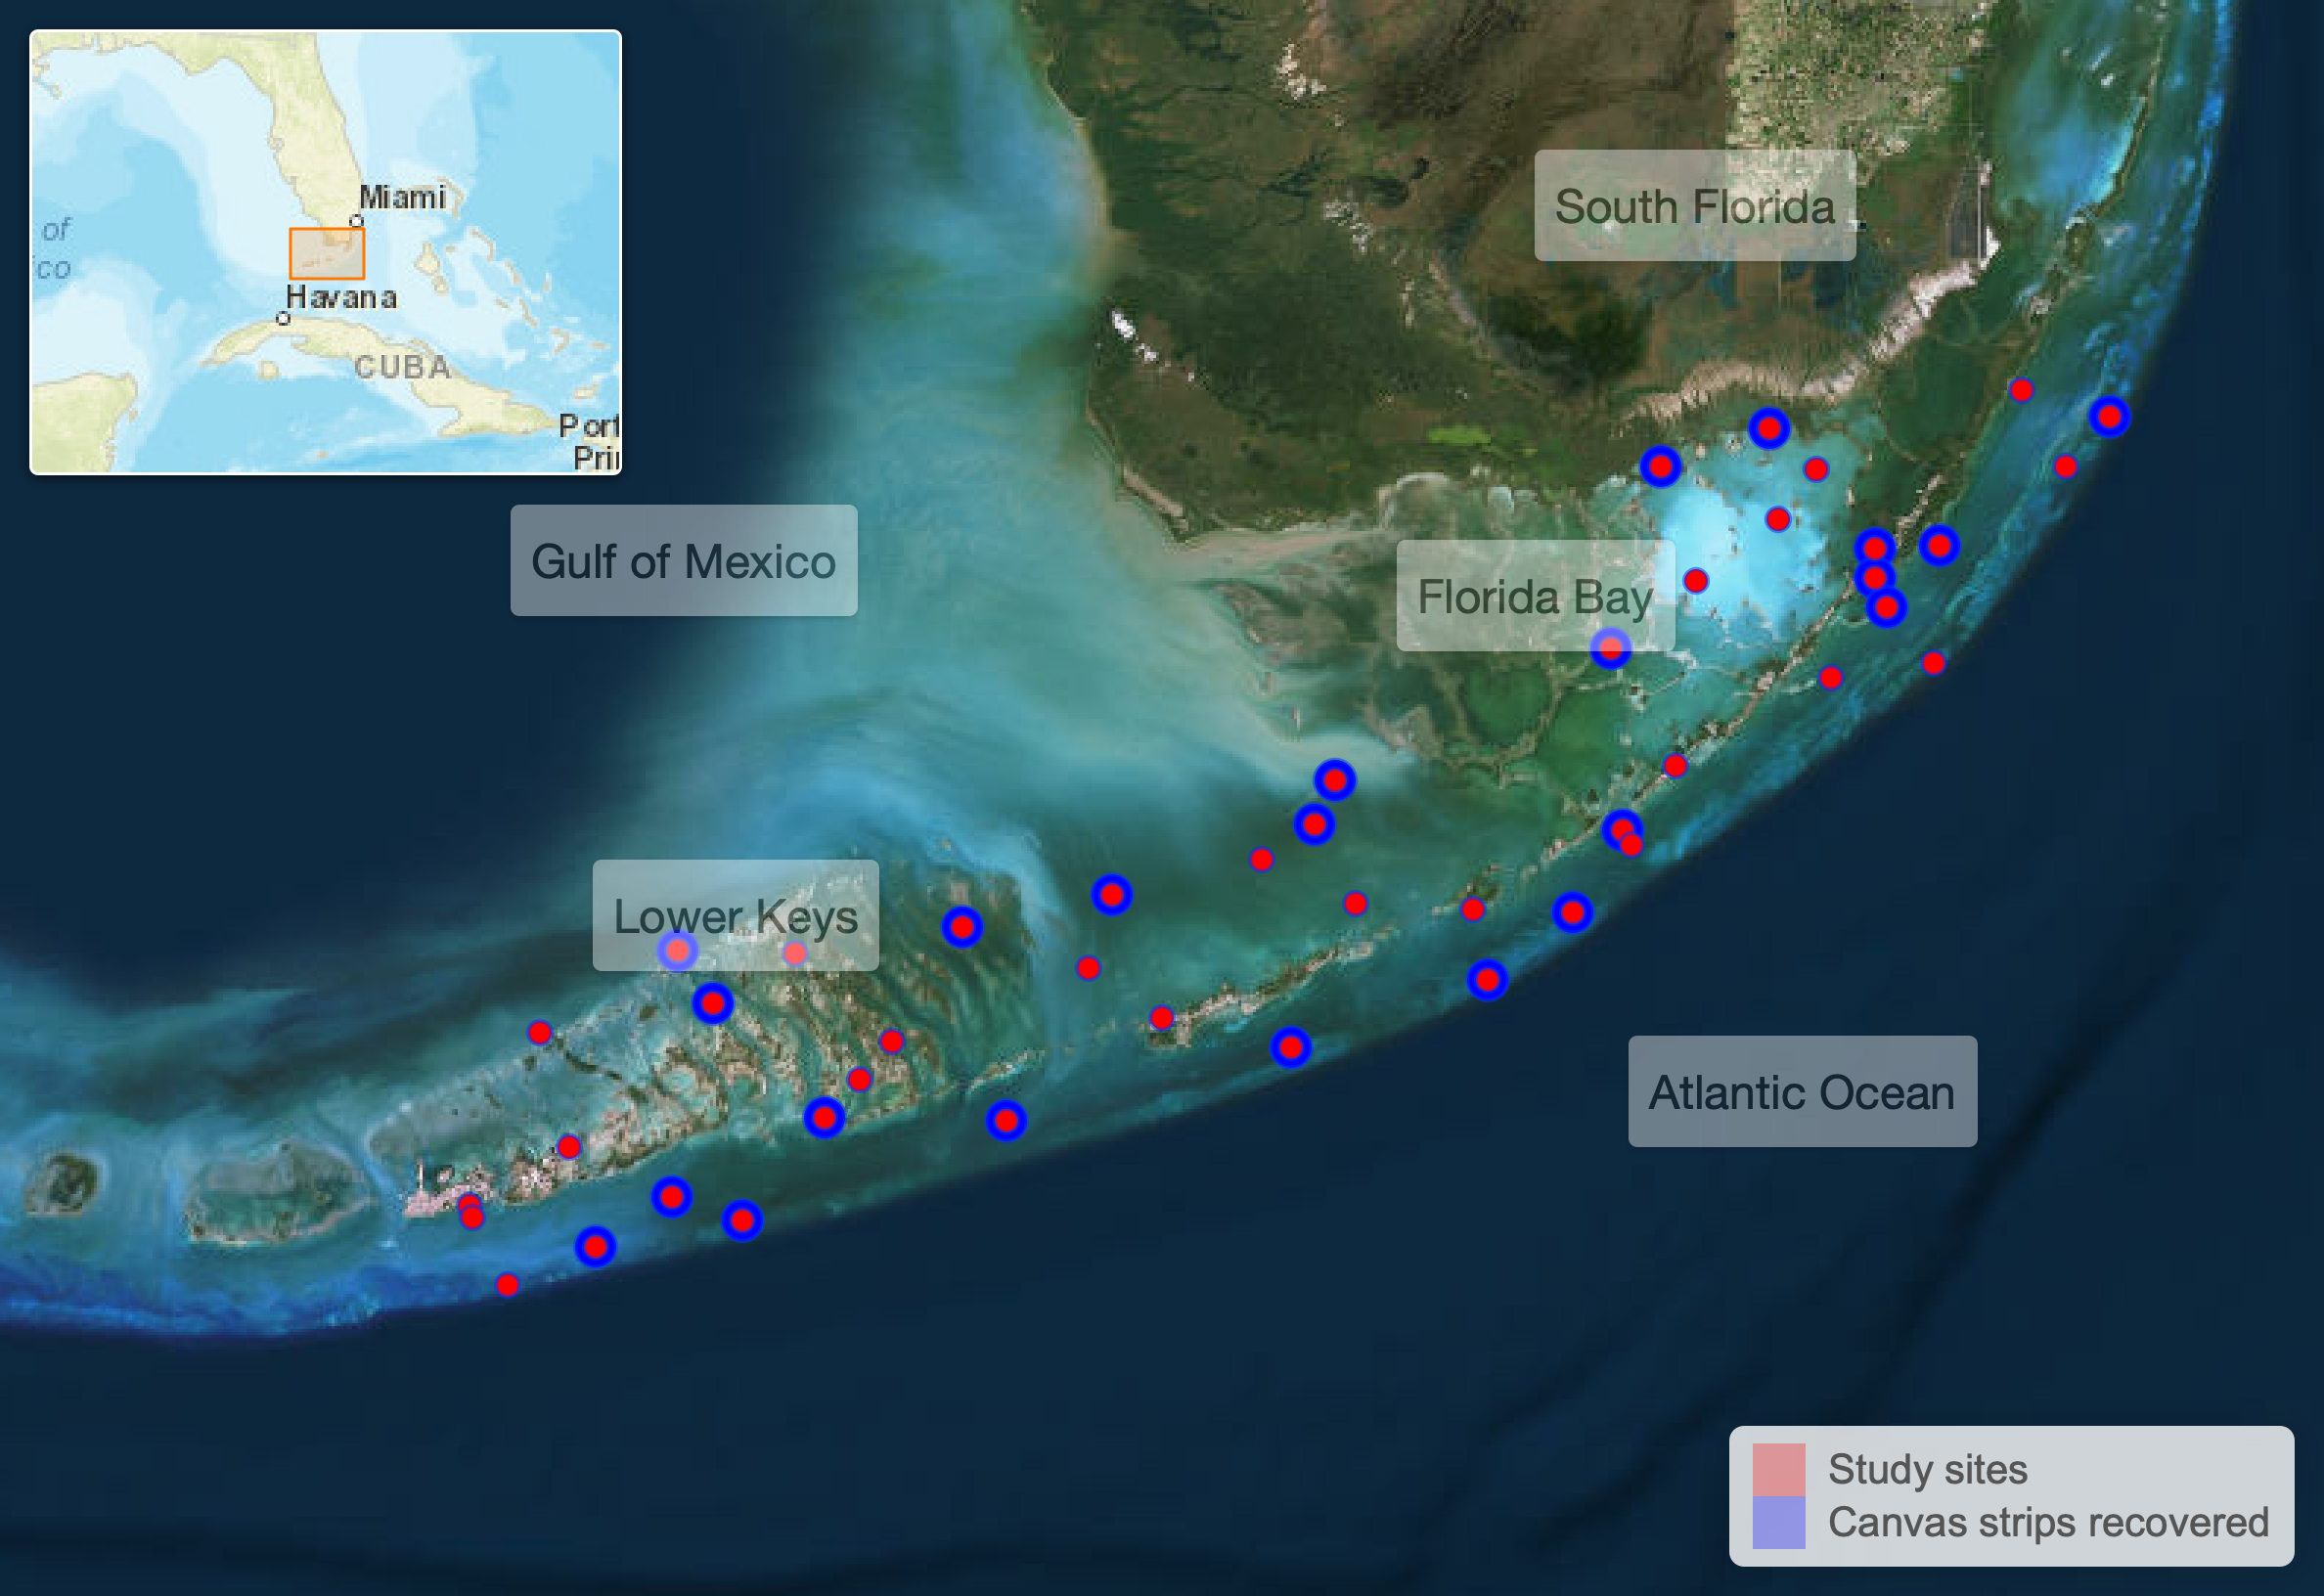
\includegraphics[width=.99\textwidth,clip, trim={0.1mm 0.1mm 0.1mm 0.1mm}]{OEM1_site_map.png}
\caption[Regional map including sites]{Map of South Florida including study sites and sites where canvas strips were successfully recovered.}
  \label{Online Resource:2F0}
\end{figure}

\begin{table}[h]
  \centering
  \caption{Modified Braun-Blanquet abundance scores, their description, and their assigned percent coverage.}
    \begin{tabular}{clc}
\hline\noalign{\smallskip}

    BB Score & \multicolumn{1}{c}{Description} & \multicolumn{1}{p{12em}}{\centering Assigned percent coverage} \\
    \noalign{\smallskip}\hline\noalign{\smallskip}
    0     & Species absent from quadrat & 0 \\

    0.1   & Species represented by a solitary short shoot, \textless{} 5\% cover  & 0.1 \\

    0.5   & Species represented by a few (\textless{} 5 ) shoots, \textless{} 5\% cover  & 0.5 \\

    1     & Species represented by many  (\textgreater{} 5)  shoots, \textless{} 5\% cover & 2.5 \\

    2     & 5\% - 25\% cover  & 15 \\

    3     & 25\% - 50\% cover  & 37.5 \\

    4     & 50\% - 75\% cover  & 62.5 \\

    5     & 75\% - 100\% cover  & 87.5 \\
        \noalign{\smallskip}\hline\noalign{\smallskip}
    \end{tabular}%
  \label{app:bbscore}%
\end{table}%







\begin{table}[ht]
  \centering
  \caption{Sediment categories and their assigned ranking of increasing coarseness}
    \begin{tabular}{ccp{22em}}
\hline\noalign{\smallskip}



    Sediment Category & Numerical Value & \multicolumn{1}{c}{\centering Description} \\
        \noalign{\smallskip}\hline\noalign{\smallskip}
    \multicolumn{1}{c}{\multirow{2}[1]{*}{Mud}}   & \multicolumn{1}{c}{\multirow{2}[1]{*}{1}}     & Individual grains indistinguishable, easily compress in hand, sediment remains clumped after compression \\
    \multicolumn{1}{c}{\multirow{2}[1]{*}{Sandy Mud}} & \multicolumn{1}{c}{\multirow{2}[1]{*}{2}}     & Majority of grains indistinguishable but textured upon touch, easily compress in hand, sediment remains clumped after compression \\
    \multicolumn{1}{c}{\multirow{2}[1]{*}{Muddy Sand}} & \multicolumn{1}{c}{\multirow{2}[1]{*}{3}}     & Sandy texture upon touch but compresses in hand, sediment dissociates upon release with most grain falling in water column  \\
    Sand  & 4     & Clearly distinguishable grains, difficult to compress in hand, grains fall quickly in water  \\
    Coarse Shell & 5     & Shell and shell remains dominate sediments (approx. 5-10 mm in size) \\
    Halimeda-Hash & 6     & Remains of carbonate segments from \textit{Halimeda} detritus (approx. 5-10 mm in size) \\
    Rubble & 7     & Medium size rock (approx. 10-25 mm in size) \\
    Live Coral & 8     & Continuous living coral \\
    Rock  & 9     & Bedrock or solid biogenic carbonate formations \\
            \noalign{\smallskip}\hline\noalign{\smallskip}
        \end{tabular}

\end{table}






\begin{figure}[ht]
  \centering
   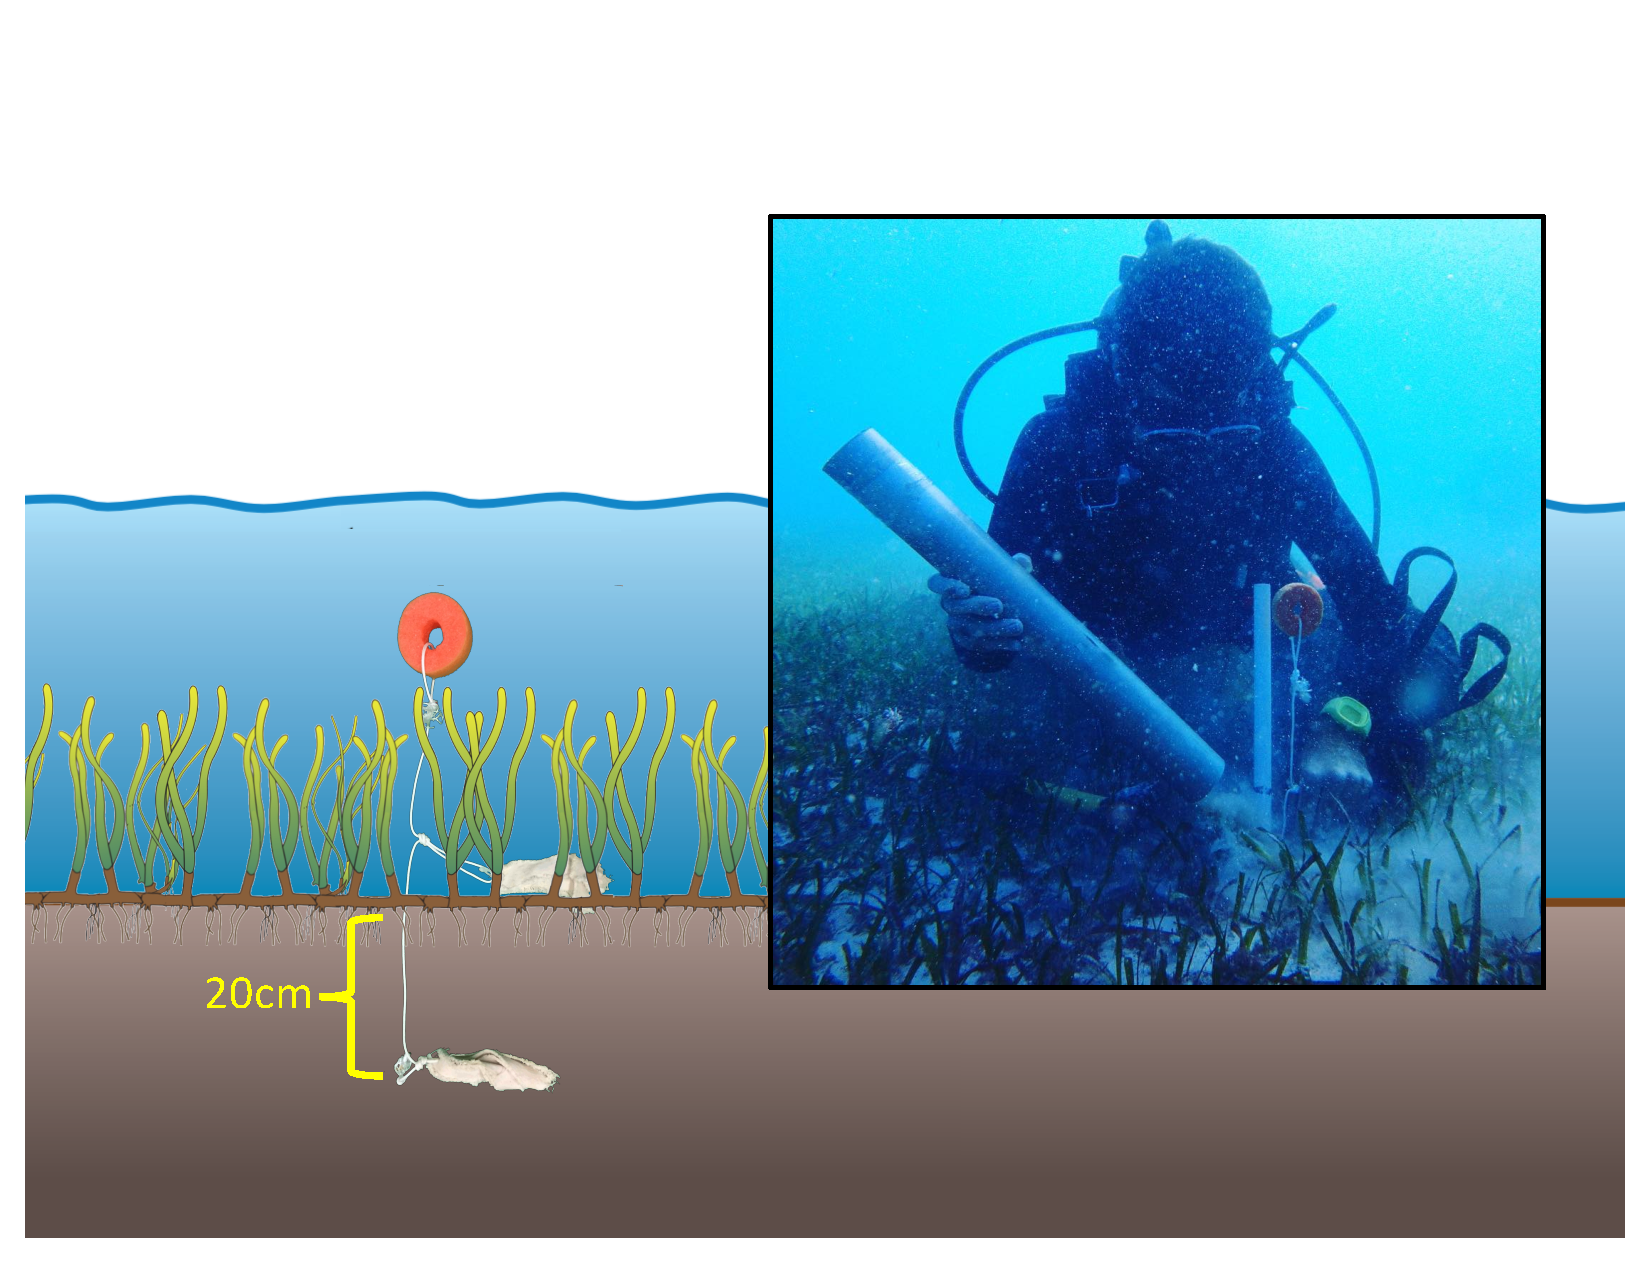
\includegraphics[width=.99\textwidth,clip, trim={1.7cm 2.5cm 1.0cm 3.2cm}]{OEM4_deployment_method}
\caption[Canvas assay deployment apparatus]{Depiction of single canvas assay deployment apparatus. Strips were deployed at each site (n = 10) at the sediment-water interface and 20 cm depth with foam buoy for easy detection.}
  \label{fig:2F1}
\end{figure}



\begin{table}[htbp]
  \centering
  \caption{Summary of sediment and seagrass characteristics measured across study sites.}
    \begin{tabular}{cccccccc}
\hline\noalign{\smallskip}

          & \multicolumn{1}{c}{\multirow{2}[1]{*}{n}}     & \multicolumn{1}{p{8em}}{Fraction of sites where present (\%)} & \multicolumn{1}{p{4em}}{\centering \multirow{2}[1]{*}{mean}} & \multicolumn{1}{p{4em}}{\centering \multirow{2}[1]{*}{SE}} & \multicolumn{1}{p{4em}}{\centering \multirow{2}[1]{*}{median}} & \multicolumn{1}{p{4em}}{\centering \multirow{2}[1]{*}{min}}   & \multicolumn{1}{p{4em}}{\centering \multirow{2}[1]{*}{max}} \\
    \noalign{\smallskip}\hline\noalign{\smallskip}

    LOI (\%) & 46    & -     & 6.9   & 0.6   & 5     & 3.3   & 19.5 \\

    C\textsubscript{org} content (\%) & 46    & -     & 2.4   & 0.2   & 1.7   & 0.7   & 8.6 \\

    dry bulk density (g cm\textsuperscript{-3}) & 46    & -     & 0.7   & 0     & 0.7   & 0.2   & 1.5 \\

    C\textsubscript{org} density (mg cm\textsuperscript{-3}) & 46    & -     & 13.8  & 0.8   & 12.9  & 6.2   & 27.7 \\

    Mud content (\%) & 45    & -     & 33.1  & 3.7   & 28    & 1.4   & 90.1 \\

    \textit{Thalassia} coverage (\%) & 46    & 93.5  & 17.8  & 2.3   & 15.6  & 0     & 60.9 \\

    \textit{Syringodium} coverage (\%) & 46    & 50    & 7.9   & 2.2   & 0.4   & 0     & 73.3 \\

    \textit{Halodule} coverage (\%) & 46    & 34.8  & 1.5   & 0.7   & 0     & 0     & 22.3 \\

    Total seagrass coverage (\%) & 46    & 95.7  & 1.5   & 0.7   & 0     & 0     & 22.3 \\

    seagass canopy ht. (cm) & 44    & -     & 18.8  & 1.2   & 17.3  & 7.9   & 41.2 \\
        \noalign{\smallskip}\hline\noalign{\smallskip}
    \end{tabular}%
  \label{tab:addlabel}%
\end{table}%


\begin{figure}[h]
  \centering
  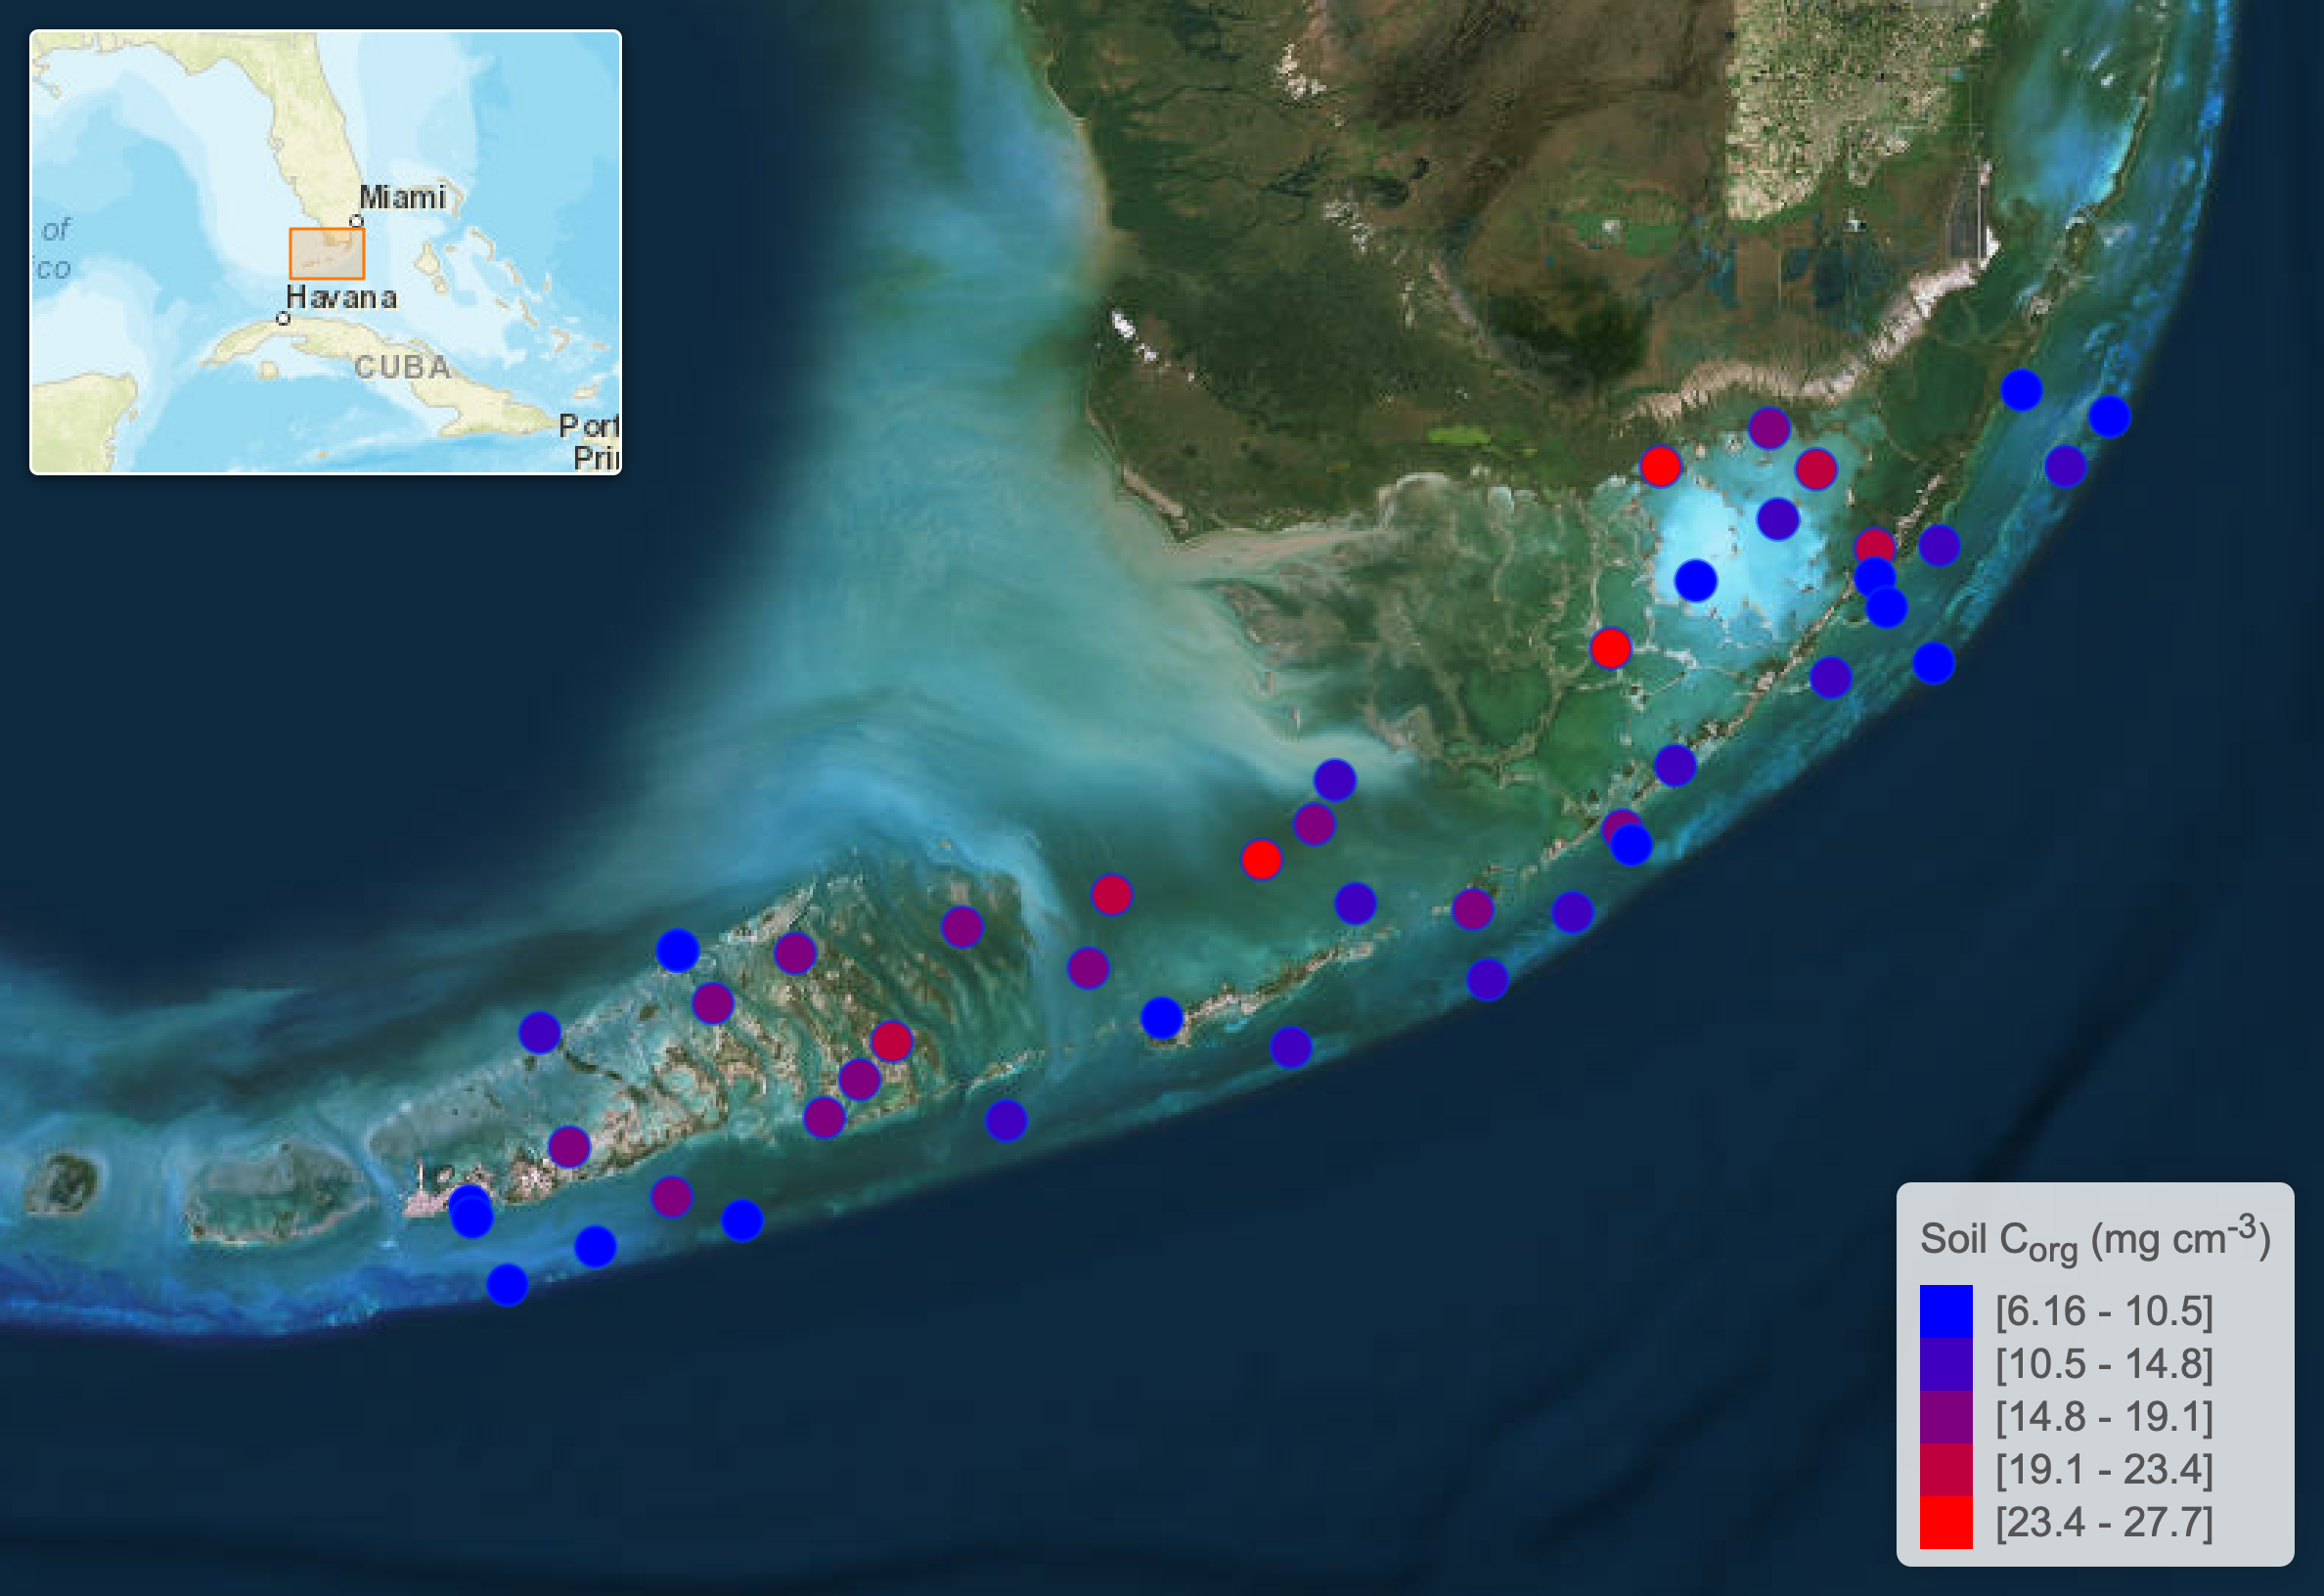
\includegraphics[width=.95\textwidth]{OEM_6_Carbon_map_A.png}   
  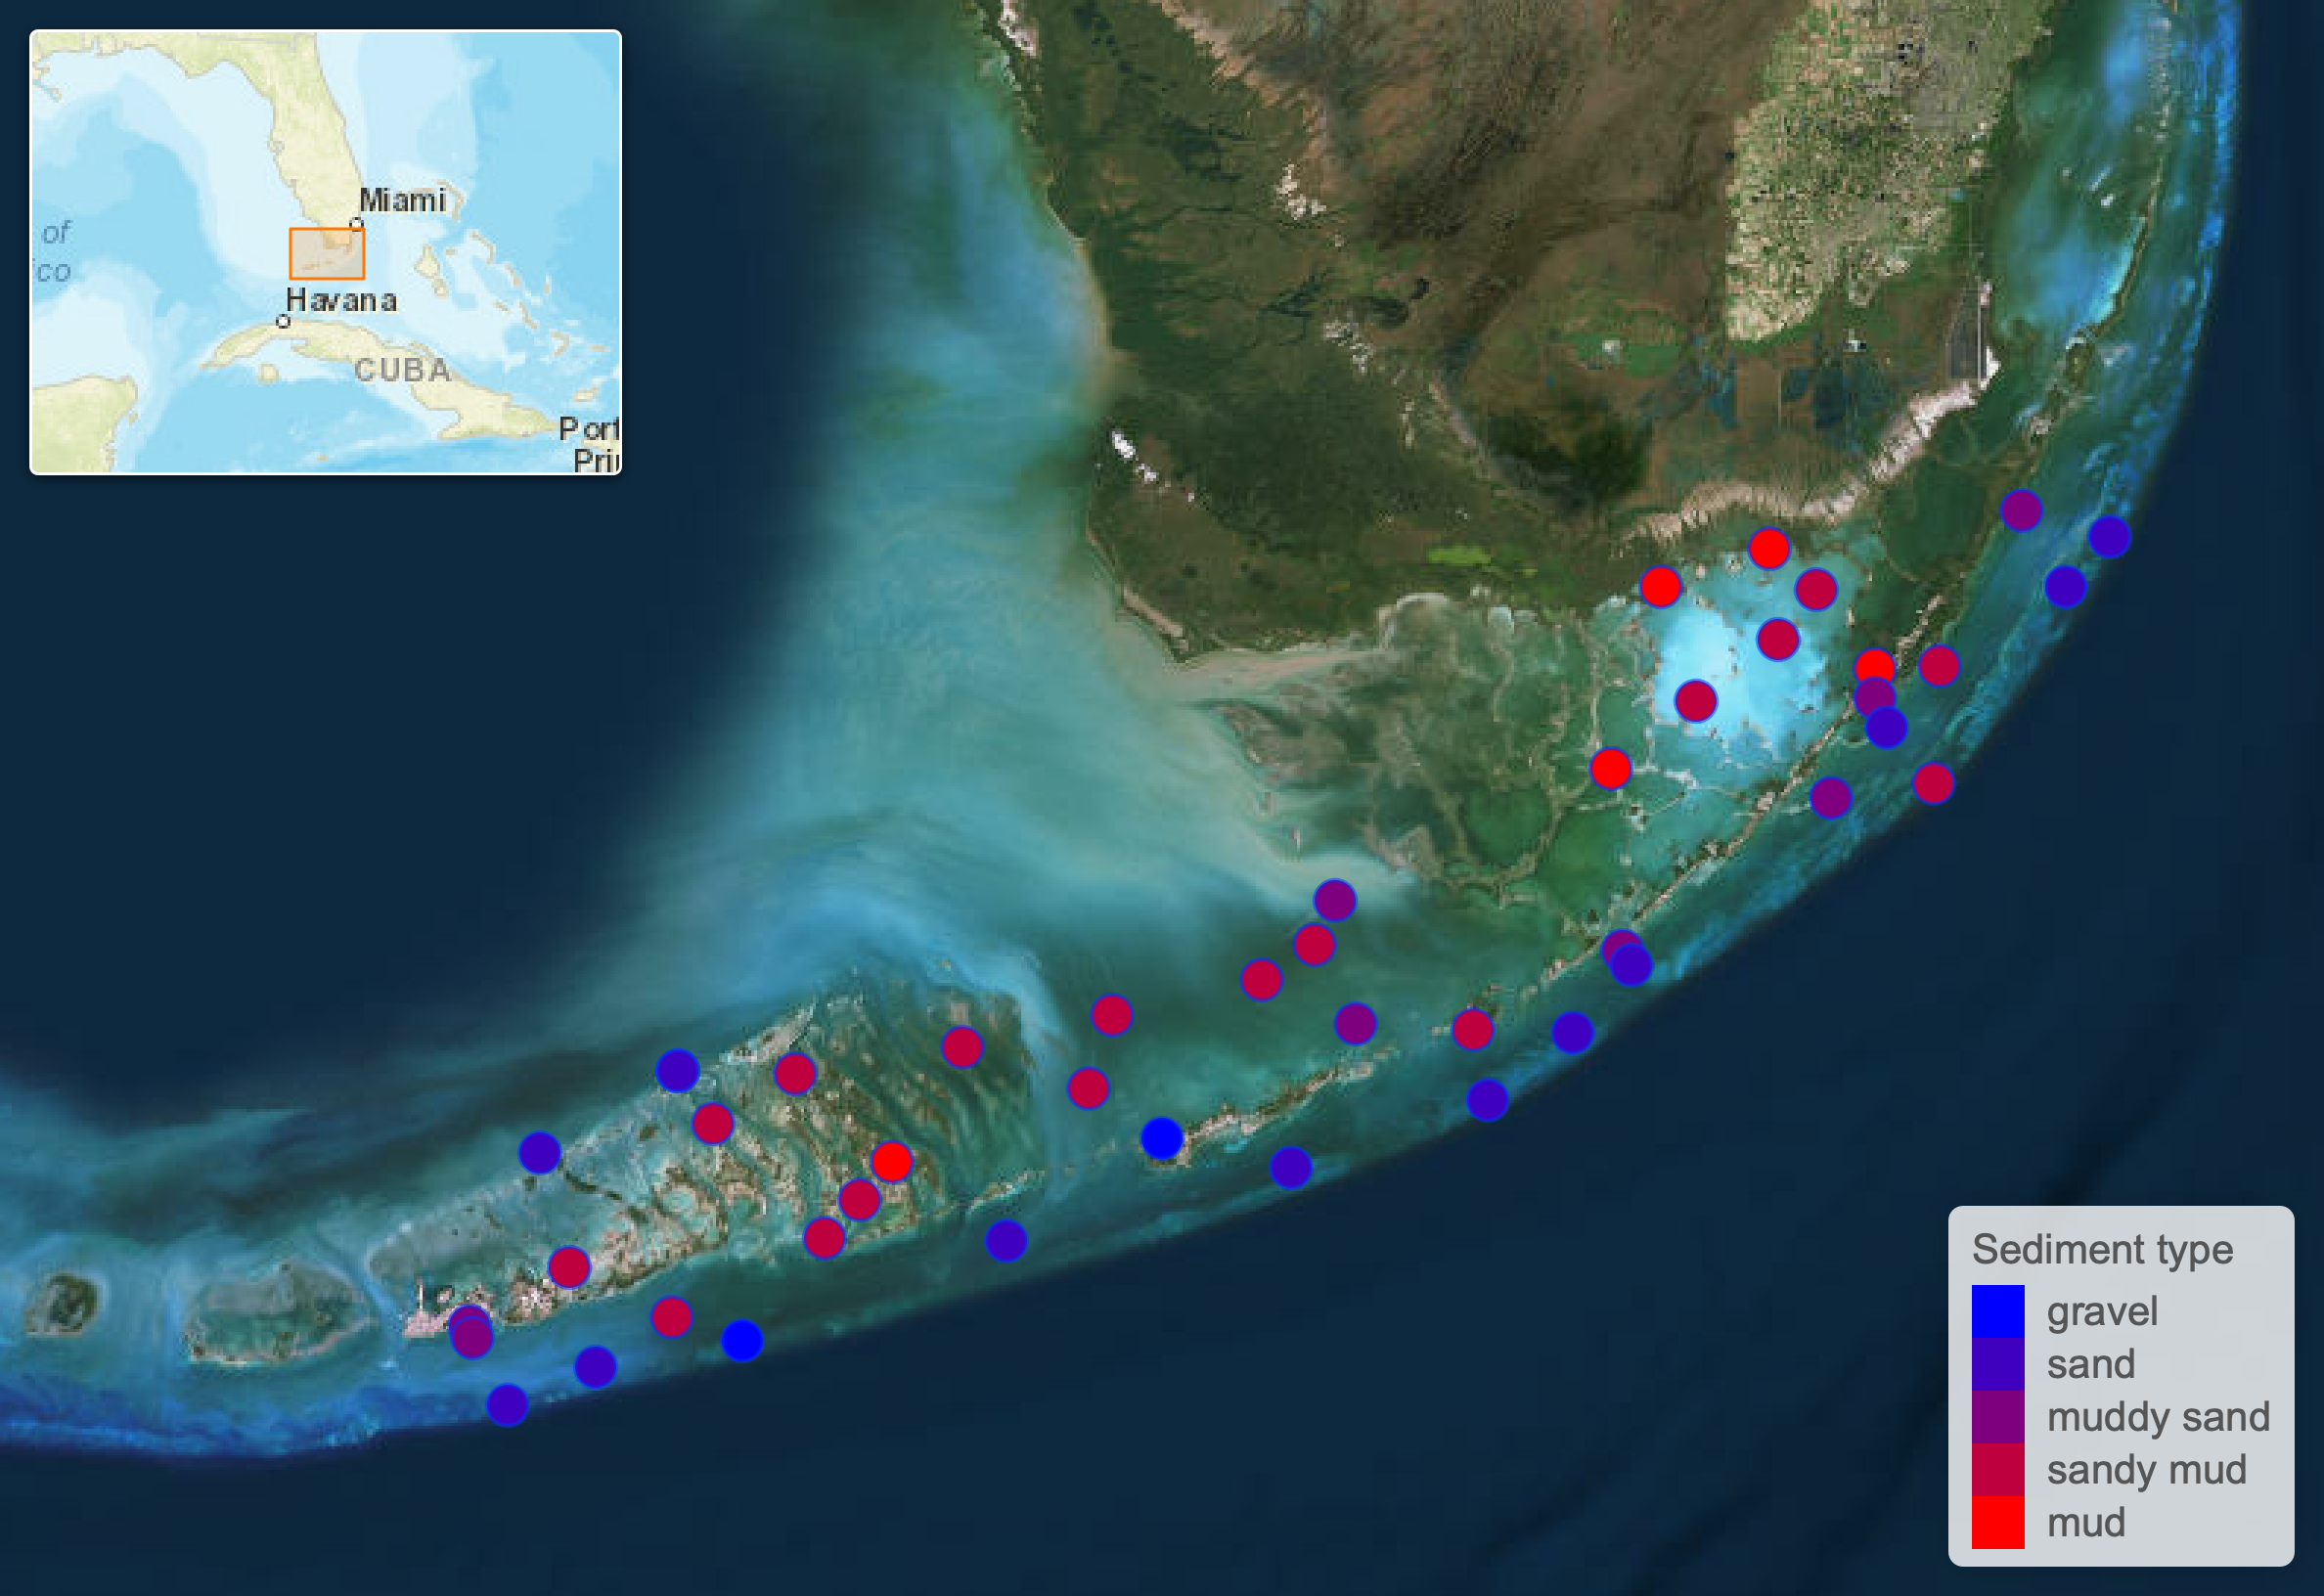
\includegraphics[width=.95\textwidth]{OEM_6_Carbon_map_B.png}
\caption[Map of sediment characteristics]{Map showing (\textit{top)} surface soil C\textsubscript{org} density, and (\textit{bottom)} sediment type across 45 study sites of Florida Bay and the Florida Keys.}
  \label{fig:2F3}
\end{figure}





% Table generated by Excel2LaTeX from sheet 'Sheet1'
\begin{table}[htbp]\small \centering
  \centering
  \caption{Summarized breakdown rates of canvas strips buried at 20 cm depth and deployed on the sediment surface}
    \begin{tabular}{lrrrrrrrrrr}
      \hline\noalign{\smallskip}
          & \multicolumn{2}{p{8em}}{\centering Tensile strength at T\textsubscript{final} (N)}     & \multicolumn{2}{p{8em}}{\centering Tensile stregth loss (\% day\textsuperscript{-1})} & \multicolumn{2}{p{6em}}{\centering Weight loss (\% day\textsuperscript{-1})} & \multicolumn{2}{p{7em}}{\centering Decay rate, \textit{k} (year\textsuperscript{-1})} & \multicolumn{2}{p{7em}}{\centering Decay rate, \textit{k} (day\textsuperscript{-1})} \\


          & \multicolumn{1}{l}{Buried} & \multicolumn{1}{l}{Surface} & \multicolumn{1}{l}{Buried} & \multicolumn{1}{l}{\centering Surface} & \multicolumn{1}{l}{Buried} & \multicolumn{1}{l}{Surface} & \multicolumn{1}{l}{Buried} & \multicolumn{1}{l}{Surface} & \multicolumn{1}{l}{Buried} & \multicolumn{1}{l}{Surface} \\

              \noalign{\smallskip}\hline\noalign{\smallskip}
              
    Mean & 18.377 & 31.508 & 0.00529 & 0.00499 & 0.0877 & 0.077 & 0.3504 & 0.3054 & 0.00096 & 0.000837 \\
    SE    & 2.683 & 6.556 & 0.00006 & 0.00018 & 0.005 & 0.0066 & 0.022 & 0.0277 & 0.00006 & 0.000076 \\
    Median & 15.948 & 16.41 & 0.00528 & 0.0052 & 0.0815 & 0.0806 & 0.3215 & 0.3178 & 0.000881 & 0.000871 \\
    Max   & 49.229 & 127.051 & 0.00603 & 0.00628 & 0.1394 & 0.1221 & 0.5854 & 0.5028 & 0.001604 & 0.001377 \\
    Min   & 2.326 & 4.138 & 0.00456 & 0.00261 & 0.051 & 0.0191 & 0.1952 & 0.0708 & 0.000535 & 0.000194 \\

\noalign{\bigskip}

\multicolumn{2}{c}{\multirow{1}[1]{*}{All sites}} &  &  & &  &  &  &  &  &  \\

    \multicolumn{1}{l}{{Mean $\pm$ SE}} & \multicolumn{2}{c}{24.942 $\pm$ 3.636} &      \multicolumn{2}{c}{0.00514 $\pm$ 0.00009} &        \multicolumn{2}{c}{0.0824 $\pm$ 0.0042} &          \multicolumn{2}{c}{0.3279 $\pm$ 0.0178} &        \multicolumn{2}{c}{0.000898 $\pm$ 0.000046} \\





        \noalign{\smallskip}\hline
    \end{tabular}%
  \label{tab:addlabel}%
\end{table}%


% Table generated by Excel2LaTeX from sheet 'appendix'

\begin{table}[htbp]\small
  \centering
  \caption{Literature review of decay rates in seagrass ecosystems}
  \renewcommand{\arraystretch}{1}
\begin{tabular}{ccccc}

  \hline\noalign{\smallskip}



    \multicolumn{1}{c}{\multirow{2}[1]{*}{Substrate}} & \multicolumn{1}{c}{\multirow{2}[1]{*}{Details}} & \multicolumn{1}{c}{\multirow{2}[1]{*}{Additional Notes}} & \multicolumn{1}{p{6em}}{\centering Breakdown rate (day \textsuperscript{-1})} & \multicolumn{1}{c}{\multirow{2}[1]{*}{Citation}} \\

    \noalign{\smallskip}\hline\noalign{\smallskip}



    \multicolumn{1}{c}{Mixed litter} & \textit{Z. marina} & Laboratory experiment & 0.004 & \citealt{Godshalk:1978vc}  \\

    \multicolumn{1}{c}{Seagrass leaves} & \textit{Z. marina} & Laboratory experiment & 0.0035 & \citealt{Harrison:1982tu} \\

    \multicolumn{1}{c}{Seagrass leaves} & \textit{Z. marina} & Laboratory experiment & 0.018 & \citealt{Harrison:1982tu}  \\

    \multicolumn{1}{c}{Seagrass leaves} & \textit{T. testudinum} & Litterbag measurements & 0.0149 & \citealt{Rublee:1982wi} \\

    \multicolumn{1}{c}{Seagrass leaves} & \textit{Z. marina} & Litterbag measurements & 0.0136 & \citealt{Pellikaan:1982vb} \\

    \multicolumn{1}{c}{Seagrass leaves} & \textit{Z. marina} & Laboratory experiments & 0.0357 & \citealt{Pellikaan:1984va} \\

    \multicolumn{1}{c}{Mixed litter} & \textit{Z. marina} & Laboratory experiments & 0.0357 & \citealt{Pellikaan:1984va} \\


    \multicolumn{1}{c}{Seagrass leaves} & \textit{Z. marina} & Litterbag measurements & 0.0124 & \citealt{Kenworthy:1984vc} \\

    \multicolumn{1}{c}{Seagrass leaves} & \textit{C. nodosa} & Litterbag measurements & 0.023 & \citealt{Kenworthy:1984vc}   \\

    \multicolumn{1}{c}{Seagrass rhyzomes} & \textit{T. testudinum} & Litterbag measurements & 0.0007 & \citealt{Kenworthy:1984vc}   \\

    \multicolumn{1}{c}{Seagrass roots} & \textit{T. testudinum} & Litterbag measurements & 0.0183 & \citealt{Kenworthy:1984vc}   \\

    \multicolumn{1}{c}{Seagrass roots} & \textit{Z. marina} & Litterbag measurements & 0.0048 & \citealt{Kenworthy:1984vc}  \\

    \multicolumn{1}{c}{Seagrass rhyzomes} & \textit{Z. marina} & Litterbag measurements & 0.0035 & \citealt{Kenworthy:1984vc}  \\


    \multicolumn{1}{c}{Seagrass leaves} & \textit{H. stipulacea} & Litterbag measurements & 0.0032 & \citealt{Wahbeh:1985vf}  \\

    \multicolumn{1}{c}{Seagrass leaves} & \textit{T. testudinum} & Litterbag measurements & 0.0048 & \citealt{Newell:1984wl} \\

    \multicolumn{1}{c}{Seagrass leaves} & \textit{T. testudinum} & Litterbag measurements & 0.0279 & \citealt{Newell:1984wl}  \\

    \multicolumn{1}{c}{Seagrass leaves} & \textit{T. testudinum} & Literature review & 0.0007 & \citealt{Harrison:1989tp} \\

    \multicolumn{1}{c}{Seagrass leaves} & \textit{Z. marina} & Literature review & 0.007 & \citealt{Harrison:1989tp} \\

    \multicolumn{1}{c}{Seagrass leaves} & \textit{T. testudinum} & Literature review & 0.017 & \citealt{Harrison:1989tp} \\

    \multicolumn{1}{c}{Seagrass leaves} & \textit{T. testudinum} & Literature review & 0.0085 & \citealt{Harrison:1989tp} \\

    \multicolumn{1}{c}{Seagrass leaves} & \textit{T. testudinum} & Literature review & 0.008 & \citealt{Harrison:1989tp} \\

    \multicolumn{1}{c}{Seagrass leaves} & \textit{P. australis} & Literature review & 0.0013 &  \citealt{Harrison:1989tp} \\

    \multicolumn{1}{c}{Seagrass leaves} & \textit{H. tasmanica} & Literature review & 0.004 & \citealt{Harrison:1989tp} \\






    \multicolumn{1}{c}{Seagrass leaves} & \textit{C. nodosa} & Laboratory experiments & 0.0039 & \citealt{Peduzzi:1991up} \\

    \multicolumn{1}{c}{Seagrass leaves} & \textit{\textit{P. oceanica} } & Litterbag measurements & 0.0088 & \citealt{Romero:1992tx}\\

    \multicolumn{1}{c}{belowground biomass } & \textit{\textit{P. oceanica} } & lepidochronology & 0.0002 & \citealt{Romero:1992tx} \\

    \multicolumn{1}{c}{belowground biomass } & \textit{\textit{P. oceanica} } & lepidochronology & 0.0006 & \citealt{Romero:1992tx} \\

    \multicolumn{1}{c}{belowground biomass } & \textit{\textit{P. oceanica} } & lepidochronology & 0.0003 & \citealt{Romero:1992tx} \\


    \multicolumn{1}{c}{Seagrass leaves} & \textit{Z. noltii} & Litterbag measurements & 0.0164 & \citealt{Bourgues:1996ti} \\

    Seagrass leaves & \textit{\textit{P. oceanica} } & \multicolumn{1}{l}{Oxygen uptake} & 0.003 & \citealt{Mateo:1996tx} \\

    Seagrass leaves & \textit{\textit{P. oceanica} } & Litterbag measurements & 0.0068 & \citealt{Mateo:1996tx}  \\

    \multicolumn{1}{c}{Seagrass leaves} & \textit{P. oceanica} & Litterbag measurements & 0.0091 & \citealt{Cebrian:1997vp}\\

    \multicolumn{1}{c}{Seagrass leaves} & \textit{Z. marina} & Litterbag measurements & 0.019 & \citealt{Cebrian:1997vp} \\

    \multicolumn{1}{c}{Seagrass leaves} & \textit{C. nodosa} & Litterbag measurements & 0.024 & \citealt{Cebrian:1997vp} \\
    \multicolumn{1}{c}{Seagrass leaves} & \textit{\textit{P. oceanica} } & Litterbag measurements & 0.0205 & \citealt{Mateo:1997uw} \\



    Seagrass leaves & \textit{\textit{C. nodosa} } & Litterbag measurements & 0.0086 & \citealt{Perez:2001ue} \\

    Seagrass leaves & \textit{\textit{C. nodosa} } & Litterbag measurements & 0.0157 & \citealt{Perez:2001ue}\\

      \multicolumn{1}{c}{Seagrass leaves} & \textit{T. testudinum} & Litterbag measurements & 0.017 & \citealt{Fourqurean:2003wh} \\

    \multicolumn{1}{c}{Seagrass rhyzomes} & \textit{T. testudinum} & Litterbag measurements & 0.0032 & \citealt{Fourqurean:2003wh} \\

    \multicolumn{1}{c}{Mangrove leaves} & R. mangle  & Litterbag measurements & 0.0064 & \citealt{Fourqurean:2003wh} \\

    \multicolumn{1}{c}{Seagrass leaves} & \textit{Z. noltii} & Litterbag measurements & 0.016 & \citealt{Machas:2006wv} \\

    \multicolumn{1}{c}{Seagrass leaves} & \textit{P. sinuosa} & Litterbag measurements & 0.0068 & \citealt{Moore:2006wq} \\

    \multicolumn{1}{c}{Seagrass leaves} & \textit{A. griffithii} & Litterbag measurements & 0.0078 & \citealt{Moore:2006wq} \\

    \multicolumn{1}{c}{Seagrass leaves} & \textit{A. antarctica} & Litterbag measurements & 0.0116 & \citealt{Moore:2006wq} \\

    \multicolumn{1}{c}{Seagrass leaves} & Mixed species & Litterbag measurements & 0.0094 & \citealt{Moore:2006wq} \\

    Seagrass leaves & \textit{Z. muelleri}  & Litterbag measurements & 0.0152 & \citealt{Nicastro:2012wf} \\

    Seagrass leaves & \textit{T. hemprichii } & Litterbag measurements & 0.011 & \citealt{Chiu:2013uy} \\

    \multicolumn{1}{c}{Seagrass rhyzomes} & \textit{T. hemprichii } & Litterbag measurements & 0.0268 & \citealt{YANO:2013ta} \\
        \multicolumn{1}{c}{Seagrass leaves} & \textit{T. hemprichii } & Litterbag measurements & 0.0394 & \citealt{YANO:2013ta} \\

    Seagrass leaves & \textit{Z. muelleri } & Litterbag measurements & 0.0055 & \citealt{TrevathanTackett:2017cn} \\

    \noalign{\smallskip}\hline

 
    \end{tabular}%
  \label{tab:addlabel}%
\end{table}%

\renewcommand\bibname{References}

\bibliographystyle{spbasic}
\bibliography{references_supplemental_material}

%\bibitem{RefJ}
% Format for Journal Reference
%Author, Article title, Journal, Volume, page numbers (year)
% Format for books
%\bibitem{RefB}
%Author, Book title, page numbers. Publisher, place (year)
% etc
%\end{thebibliography}

\end{document}
% end of file template.tex

